\section{Experiments and Results}
\label{sec:experiments}

To evaluate the efficacy of the proposed mathematical scale restoration, we conduct experiments across two distinct regimes: highly intermittent retail demand (M5) \cite{m5} and dense, continuous sensor data (ETTm2) \cite{informer}. We benchmark \textit{ScaleRAG} against zero-shot target-only foundation models and state-of-the-art neural retrieval (TS-RAG).

All splits are strictly chronological. On M5, the held-out test window \texttt{d\_1914--d\_1941} was frozen before any test evaluation, opened exactly once, and never used to tune any component; the success criteria reported in Sec.~\ref{sec:m5-caveats} were pre-registered prior to that run. On ETTm2 the fused configuration (mean scaling, $k=20$, $w=0.25$) was selected on the validation split alone. Every retrieval candidate satisfies the horizon guard $t_r + H < \text{origin}$, so no retrieved continuation can overlap the forecast window it informs.

\begin{figure*}[t]
  \centering
  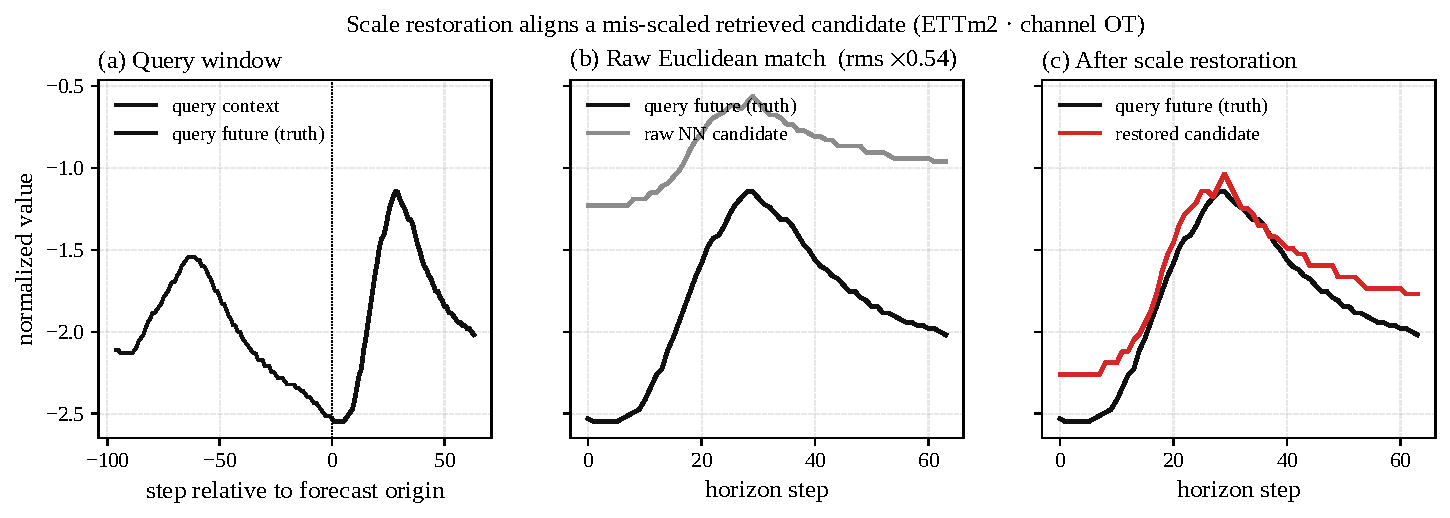
\includegraphics[width=\textwidth]{../docs/figures/fig1_motivation.pdf}
  \caption{The catastrophic scale-mismatch failure mode on real ETTm2 data. A query
    window (left) is matched against its top-1 raw-Euclidean candidate (centre), whose
    continuation tracks the query's future \emph{shape} but sits at an entirely different
    \emph{magnitude}; explicit restoration (right) maps that continuation onto the query's
    own scale using only the query context statistics.}
  \label{fig:motivation}
\end{figure*}

\subsection{The Scale Mismatch Ablation}
\label{sec:ablation}
Our primary hypothesis is that raw Euclidean retrieval on unscaled data suffers from a catastrophic magnitude mismatch, illustrated on a real query--candidate pair in Fig.~\ref{fig:motivation}. As shown in our evaluations, executing statistical k-NN on the sparse M5 dataset without scale restoration yields an unusable RMSSE of 2.7884. By explicitly reconstructing the retrieved continuation's magnitude, we prevent this catastrophic degradation, reducing RMSSE to 0.7425---a 3.8$\times$ recovery in predictive accuracy.

This mechanism transfers universally across modalities. On the dense ETTm2 benchmark, the restored retrieval candidate significantly outperformed the raw Euclidean candidate, yielding an +85.4\% MSE improvement (95\% CI: [+85.2, +85.6]) across all channels. Table~\ref{tab:ablation} reports both regimes side by side, and Fig.~\ref{fig:ablation} resolves the ETTm2 result per channel: all 7/7 channels improve, so the aggregate is not driven by a single outlier.

% Table 2: Scale-restoration ablation, raw vs. restored retrieval, on two datasets and
% two metrics (RMSSE on M5, MSE on ETTm2 -- metrics are not comparable across rows, only
% within each dataset's own raw-vs-restored pair).
% Source (M5): docs/ablation-report.md, "normalization without restoration" vs.
%              "mean scaling (+restore)", 1,000-series M5 validation split.
% Source (ETTm2): docs/scalerag-native-dev-results.json, test_mechanisms.A_restoration
%                 (frozen config scale=mean, k=20; test split, n=80,199 windows,
%                 paired-bootstrap 95% CI, window-level).
\begin{table}[t]
  \centering
  \caption{Scale restoration is decisive on both datasets. Raw retrieval normalises context
    windows for matching but does not rescale the retrieved continuation; restored retrieval
    additionally rescales candidate$\to$query before use (Sec.~\ref{sec:method}). M5 reports
    RMSSE (lower is better, no CI available for this legacy ablation); ETTm2 reports MSE with
    a paired-bootstrap 95\% CI (2,000 resamples, $n=80{,}199$ windows, 7/7 channels improved).
    Relative improvement $= (\mathrm{raw} - \mathrm{restored}) / \mathrm{raw}$; positive throughout.}
  \label{tab:ablation}
  \begin{tabular}{@{}llccc@{}}
    \toprule
    Dataset & Metric & Raw retrieval & Restored retrieval & Relative improvement \\
    \midrule
    M5 (1k, val)    & RMSSE & 2.7884 & 0.7425 & $+73.4\%$ (3.8$\times$ lower) \\
    ETTm2 (test)    & MSE   & 2.9989 & 0.4376 & $+85.4\%$ \; [$+85.2\%$, $+85.6\%$] \\
    \bottomrule
  \end{tabular}
\end{table}


\begin{figure*}[t]
  \centering
  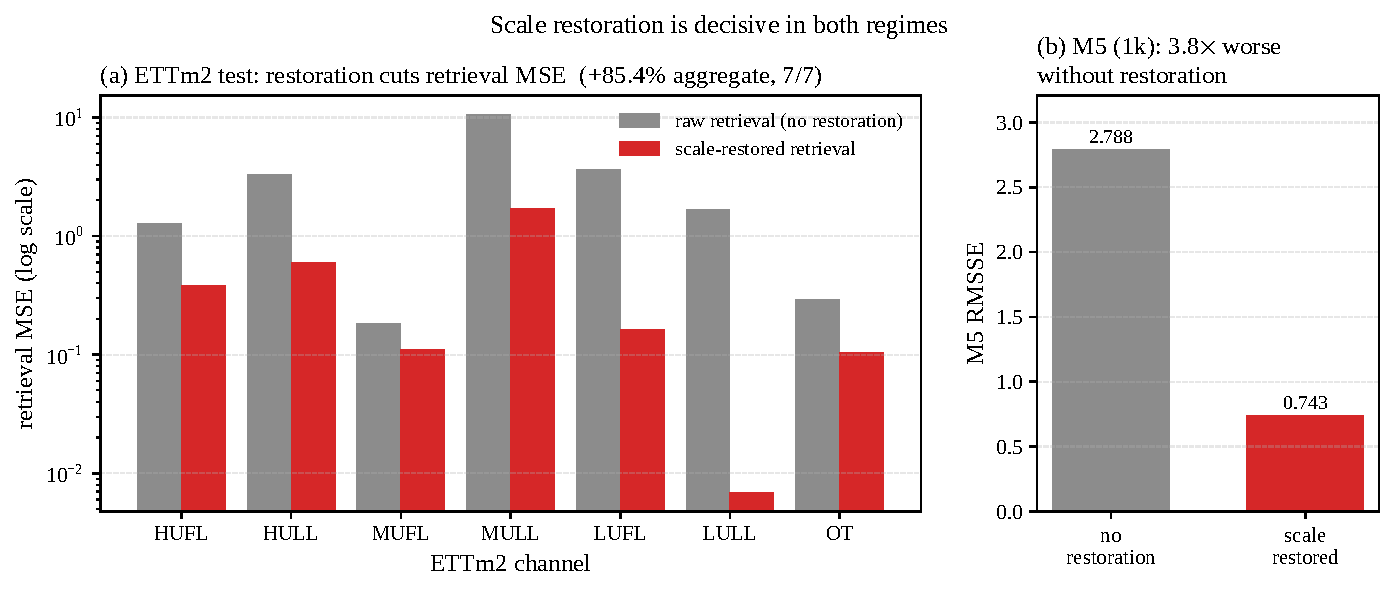
\includegraphics[width=\textwidth]{../docs/figures/fig2_ablation.pdf}
  \caption{Per-channel raw versus restored retrieval MSE on the ETTm2 test split
    ($n=80{,}199$ windows). Scale restoration improves every one of the seven channels;
    the aggregate +85.4\% is not an artefact of averaging over a single dominant series.}
  \label{fig:ablation}
\end{figure*}

\begin{figure}[t]
  \centering
  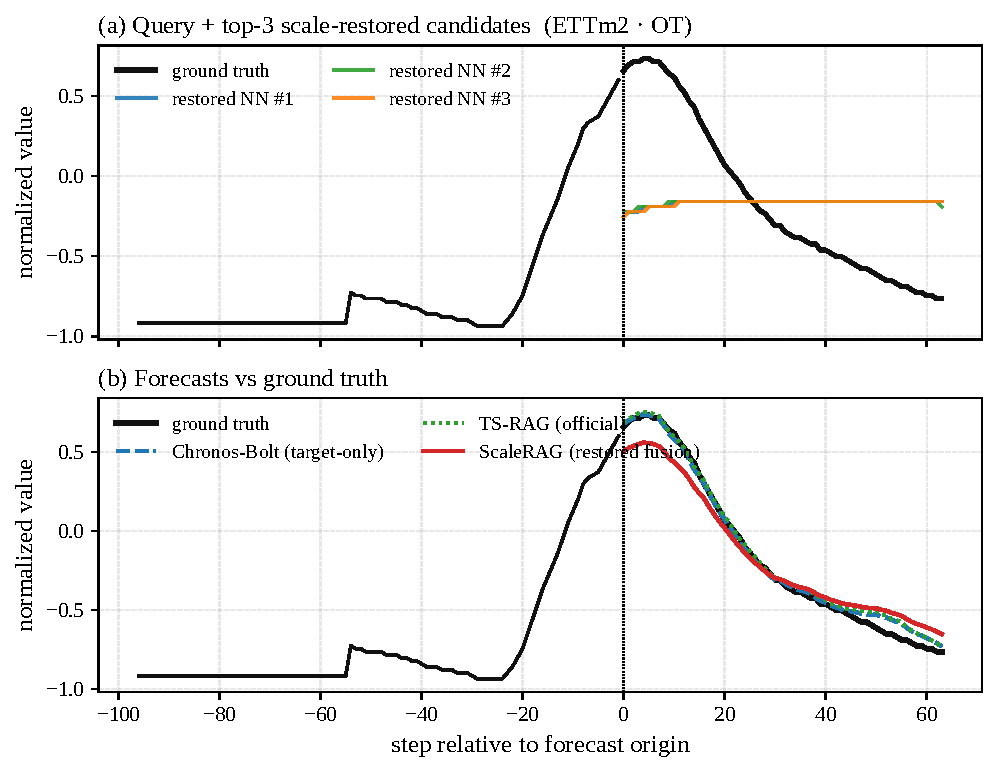
\includegraphics[width=\columnwidth]{../docs/figures/fig3_qualitative.pdf}
  \caption{Qualitative forecasts on the ETTm2 OT channel (mean scaling, $k=20$). The
    restored continuation is structurally well aligned with the ground-truth future, which
    is why the mechanism-level ablation succeeds even where the end-to-end fusion does not.}
  \label{fig:qualitative}
\end{figure}

\subsection{Regime Taxonomy and Boundary Conditions}
\label{sec:regimes}
While scale restoration definitively fixes statistical retrieval quality, its impact on the final end-to-end forecast is heavily regime-dependent. Fig.~\ref{fig:regimes} plots the realised utility of retrieval augmentation against the zero-fraction of each dataset and makes the trend explicit: the benefit grows with sparsity and scale heterogeneity, and vanishes on dense continuous channels.

On the sparse, scale-heterogeneous M5 dataset, ScaleRAG improved the frozen Chronos-2 backbone by +5.49\% RMSSE (paired-bootstrap 95\% CI [+5.40\%, +5.59\%], full 30,490-series panel). In this regime, target-only models struggle with zero-inflation and severe intermittency, making the restored historical continuations valuable. Sec.~\ref{sec:m5-caveats} qualifies this number against the pre-registered criteria.

Conversely, on the continuous ETTm2 benchmark, the neural target-only backbone (Chronos-Bolt) is remarkably strong. While our restored candidates were structurally accurate (Fig.~\ref{fig:qualitative}), fusing them with the backbone resulted in a marginal but statistically significant degradation ($-0.85\%$ MSE, 95\% CI [$-1.39\%$, $-0.28\%$]) compared to the target-only baseline. Furthermore, the official TS-RAG neural adapter outperformed our statistical fusion by 2.30\% MSE. Table~\ref{tab:main-results} summarises the ETTm2 comparison.

% Table 1: Main results on ETTm2 (context 512, horizon 64), test split, 80,199 windows.
% Metrics computed in the train-only-StandardScaler-normalised space, matching TS-RAG's
% own protocol. ScaleRAG uses the frozen dev-selected config (scale=mean, k=20, weight=0.25),
% selected on the ETTm2 validation split only, before this test split was touched (see
% docs/phase11b-preregistration.md).
% Source: reports/phase11a/repro_chronos_bolt_target_ettm2.json,
%         reports/phase11a/repro_tsrag_official_ettm2.json,
%         reports/phase11a/scalerag_native_ettm2_test.json,
%         docs/scalerag-native-dev-results.json (paired-bootstrap 95% CIs, n=80,199 windows).
% Note: the TS-RAG delta is TS-RAG's own reported point-estimate improvement over its
% backbone (reproduced to <=0.10% of the published TS-RAG numbers; no independent bootstrap
% CI was computed for this pair). The ScaleRAG deltas ARE from our own paired bootstrap
% (2,000 resamples, window-level) and are the only CIs in this table (rule: no significance
% claim without a valid CI).
% Layout: two-column journal style (svjour3 twocolumn) -- spans both columns via table*.
\begin{table*}[t]
  \centering
  \caption{Main results on ETTm2 (test, $n=80{,}199$ windows). $\Delta$MSE is the relative
    change vs.\ target-only Chronos-Bolt (positive = improvement). ScaleRAG's $\Delta$ values
    carry a paired-bootstrap 95\% CI (window-level, $n=80{,}199$); both CIs exclude zero.
    The TS-RAG $\Delta$ is its own reproduced point estimate (no CI computed here).}
  \label{tab:main-results}
  \begin{tabular}{@{}lccc@{}}
    \toprule
    Method & MSE $\downarrow$ & MAE $\downarrow$ & $\Delta$MSE vs.\ target-only \\
    \midrule
    Chronos-Bolt (target-only, frozen) & 0.1486 & 0.2235 & --- \\
    TS-RAG (official ARM)              & 0.1465 & 0.2230 & $+1.41\%$ (point estimate) \\
    ScaleRAG (restored fixed fusion)   & 0.1498 & 0.2407 & $-0.85\%$ \; [$-1.39\%$, $-0.28\%$] \\
    \bottomrule
  \end{tabular}
\end{table*}


\begin{figure}[t]
  \centering
  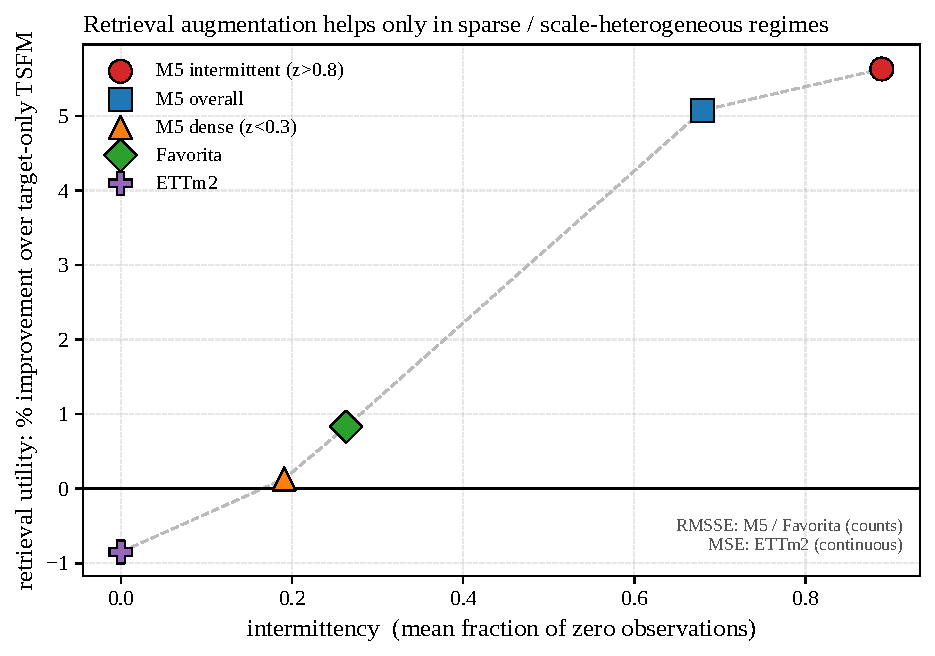
\includegraphics[width=\columnwidth]{../docs/figures/fig4_regimes.pdf}
  \caption{Taxonomy of retrieval regimes. Realised utility of retrieval augmentation over
    the target-only foundation model, plotted against dataset zero-fraction (M5 and
    Favorita in RMSSE, ETTm2 in MSE). Retrieval augmentation pays off in sparse,
    scale-heterogeneous regimes and is neutral-to-harmful on dense continuous channels.}
  \label{fig:regimes}
\end{figure}

\subsection{Held-Out M5 Evaluation: Pre-Registered Criteria and Negative Findings}
\label{sec:m5-caveats}
We report the held-out M5 outcome in full, including the results that do not favour our method. The +5.49\% RMSSE gain over the frozen Chronos-2 backbone is real and its confidence interval excludes zero, but it does \emph{not} generalise into a claim of state-of-the-art forecasting accuracy, for four reasons.

First, the margin over the strongest simple baseline is small. Against LightGBM \cite{lightgbm}, ScaleRAG improves RMSSE by only +0.69\% (95\% CI [+0.57\%, +0.82\%]). Our pre-registered success criterion required at least a 3\% relative improvement over the strongest matched baseline, so this criterion \textbf{fails} despite the interval excluding zero. Statistical significance here is not practical significance: with 30,490 series, a sub-1\% effect is comfortably detectable while remaining operationally negligible.

Second, ScaleRAG \emph{loses the official M5 metric}. On WRMSSE---the dollar-weighted, hierarchical metric that defines the M5 competition---LightGBM (0.8663) and even Seasonal-Naive (0.8697) beat ScaleRAG (1.2231). Our method is mid-pack on the benchmark's own headline metric.

Third, the RMSSE gain does not carry over to absolute-error or probabilistic accuracy. The frozen target-only Chronos-2 backbone is the best model on MASE (0.893 vs.\ our 1.020), WAPE (0.665 vs.\ 0.698), MAE (0.960 vs.\ 1.008), pinball loss (0.289 vs.\ 0.298), and calibration: at a nominal 80\% level, Chronos-2 attains 0.786 empirical coverage while our gated fusion under-covers at 0.698. Retrieval fusion therefore trades typical-case and distributional accuracy for reduced large squared errors on intermittent series.

Fourth, taken together, \textbf{0 of 3 pre-registered success criteria were met} on the held-out panel. We report this rather than re-tuning, because the test split was consumed exactly once by design and any post-hoc adjustment would invalidate it.

The honest reading is that no single method dominates: the winner reorders with the metric. This metric-dependent reordering, rather than a leaderboard position, is the empirical contribution---together with the mechanism-level result of Sec.~\ref{sec:ablation}, which is unambiguous and holds in both regimes.

\subsection{Compute and Efficiency Trade-offs}
\label{sec:compute}
TS-RAG achieves superior accuracy on continuous data but introduces 4.78M trainable parameters and significant VRAM overhead. ScaleRAG's retrieval and restoration stages introduce \emph{zero} trainable parameters; on M5 the only trained component is the LightGBM gate of Sec.~\ref{sec:fusion}, which is orders of magnitude smaller than a neural mixer and requires no pretraining corpus.

Search is \emph{exact} in every configuration reported here---we never approximate the nearest-neighbour set, so accuracy differences cannot be attributed to index quantisation. Two exact implementations are used, matched to scale. The ETTm2 study uses FAISS with a flat CPU-resident \texttt{IndexFlatL2}, which is why Table~\ref{tab:compute} attributes 0\,MB VRAM and 0.607\,ms per window to the retrieval step. Scaling to the full 30,490-series M5 panel makes the CPU path intractable ($\mathcal{O}(n_{\text{query}} \times n_{\text{candidate}})$ at roughly five hours per origin), so for that panel we use a batched GPU implementation of the \emph{same} exact search: the GPU performs a coarse float32 $L_2$ over-fetch, and the final top-$k$ selection, tie-break, and float64 restoration are resolved exactly as in the CPU path. This GPU path was verified bit-for-bit identical to the frozen CPU retriever before any held-out run (maximum absolute difference 0.0); it is an arithmetic acceleration, not a method change.

Table~\ref{tab:compute} gives the full accounting and Fig.~\ref{fig:pareto} plots the resulting accuracy--latency trade-off: on ETTm2, ScaleRAG is Pareto-dominated, being both slower end-to-end (1.038\,ms vs.\ 0.450\,ms per window) and less accurate than the official neural adapter. Fig.~\ref{fig:sensitivity} shows that this conclusion is not an artefact of the neighbour budget---restored-retrieval and fused MSE are stable across $k \in \{5, 10, 20\}$.

% Table 3: Measured compute / storage / parameter accounting, one machine (RTX 5070 Ti,
% sm_120), batch 256, warm-up excluded from all timings.
% Source: reports/phase11a/compute_backbone.json (backbone params/VRAM/latency),
%         reports/phase11a/compute_scalerag.json (ScaleRAG retrieval index/latency/RAM),
%         reports/phase11a/repro_{chronos_bolt_target,tsrag_official}_ettm2.json
%         (full-test wall-clock eval_seconds, used to derive the TS-RAG per-window latency
%         by scaling the measured backbone latency by the wall-clock ratio -- the ARM
%         adds ~4.3% wall time over the frozen backbone).
% ScaleRAG's "storage" is its train-only in-RAM float64 index (contexts + continuations);
% the official TS-RAG knowledge-base pickle (1,528.6 MB, full-series, not train-only) is
% listed alongside it as an unlike-for-unlike storage reference, not a fair comparison
% (ScaleRAG deliberately restricts to a stricter, train-only candidate pool).
% Requires \usepackage{graphicx} for \resizebox (wide 6-column table).
% Layout: two-column journal style (svjour3 twocolumn) -- spans both columns via table*.
% Inside table*, \textwidth is the full two-column text width, so \resizebox{\textwidth}
% constrains the tabular to the spread exactly (in a single-column table it would have
% overflowed the column by ~half the page).
\begin{table*}[t]
  \centering
  \caption{Measured compute, storage, and trainable-parameter accounting (ETTm2, one machine,
    batch 256, warm-up excluded). ScaleRAG's retrieval index is CPU-resident (0 VRAM);
    latency is reported separately for the frozen backbone forward pass and the retrieval
    step, since ScaleRAG's fused forecast requires both.}
  \label{tab:compute}
  \resizebox{\textwidth}{!}{%
  \begin{tabular}{@{}lccccc@{}}
    \toprule
    Component & Train.\ params & Latency / window & Peak VRAM & Peak RAM & Storage \\
    \midrule
    Chronos-Bolt backbone (frozen) & 0 (205.3M) & 0.431\,ms & 1{,}562\,MB & --- & --- \\
    TS-RAG ARM (official)          & 4.78M      & 0.450\,ms ($+4.3\%$) & $\sim$1.6\,GB & --- & 1{,}528.6\,MB$^{\ast}$ \\
    ScaleRAG retrieval (non-neural) & 0          & 0.607\,ms (CPU) & 0 (CPU) & 1{,}245.0\,MB & 1{,}096.2\,MB \\
    \midrule
    ScaleRAG total (backbone + retrieval) & 0 & 1.038\,ms & 1{,}562\,MB & 1{,}245.0\,MB & --- \\
    \bottomrule
  \end{tabular}%
  }
  \\[4pt]
  {\footnotesize $^{\ast}$Full-series official knowledge base (not train-only); listed for
   storage reference, not a like-for-like index-size comparison.}
\end{table*}


\begin{figure}[t]
  \centering
  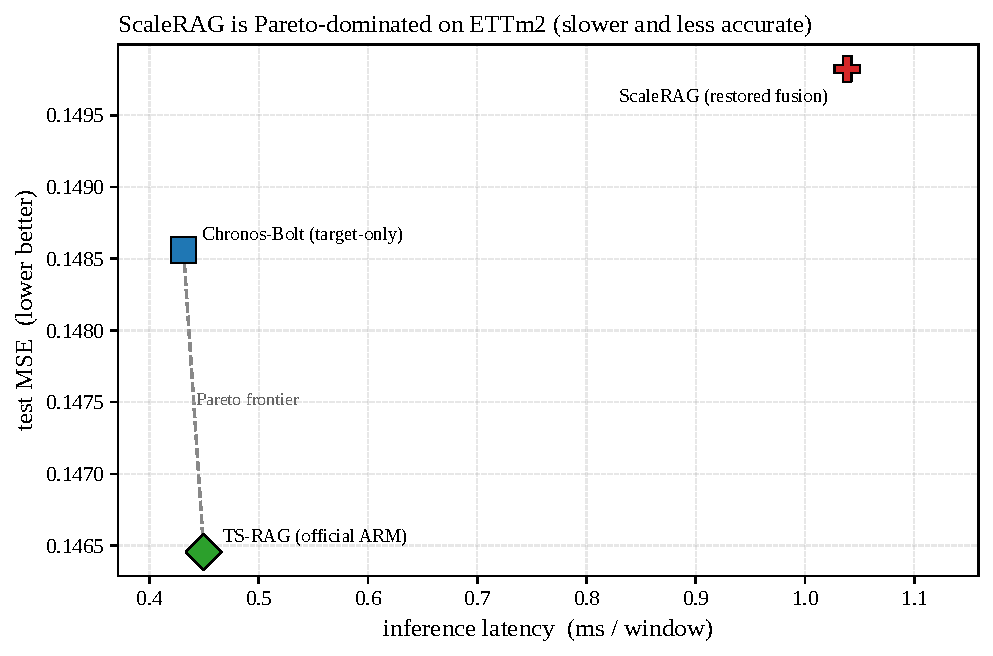
\includegraphics[width=\columnwidth]{../docs/figures/fig5_pareto.pdf}
  \caption{Accuracy versus latency per window on ETTm2. ScaleRAG is Pareto-dominated in
    this regime: the official TS-RAG adapter is both faster end-to-end and more accurate.
    The efficiency argument for ScaleRAG rests on trainable-parameter count and
    deployability, not on wall-clock latency.}
  \label{fig:pareto}
\end{figure}

\begin{figure}[t]
  \centering
  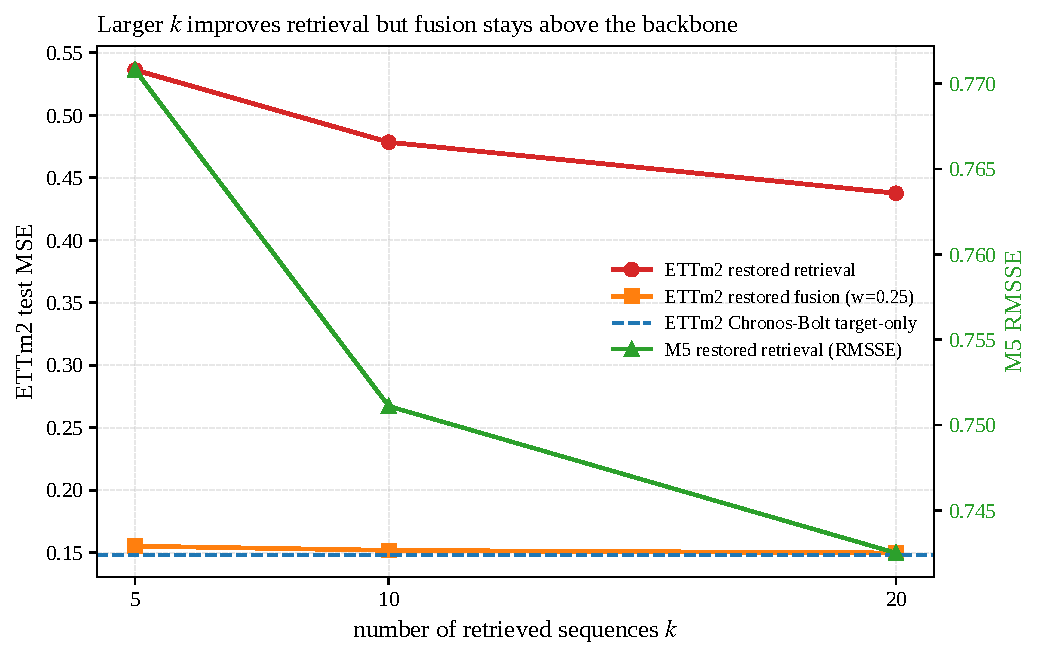
\includegraphics[width=\columnwidth]{../docs/figures/fig6_sensitivity.pdf}
  \caption{Sensitivity to the neighbour budget $k \in \{5, 10, 20\}$ on ETTm2 (mean
    scaling, fusion weight $0.25$). Both restored-retrieval and fused MSE are flat in $k$,
    so the reported outcome is not an artefact of the frozen $k=20$ choice.}
  \label{fig:sensitivity}
\end{figure}

Therefore, explicit statistical restoration is not proposed as a substitute for neural RAG on dense benchmarks, but rather as an operational option for sparse datasets and resource-constrained environments where neural adapters risk scale hallucination, cannot be pretrained, or are impossible to deploy.
